\begin{problem}[1]
  Let $D$ be the triangle with vertices $(-1, 1)$, $(1, -2)$, and $(3, 4)$.
  \begin{enumerate}
    \item Let $S$ be the triangle with vertices $(0, 0)$, $(1, 0)$, and $(1,
      1)$. Find a change of variables that maps $S$ to $D$.

      Note: Since the change of variable will preserve the boundary as lines,
      the transformation is affine. That is, $x = g(u, v)$ and $y = h(u, v)$
      where $g(u, v) = a_1u + a_2v + a_3$ and $h(u, v) = b_1u + b_2v + b_3$ for
      constants $a_n$ and $b_n$, $n = 1, 2, 3$.

    \item Use the change of variable to evaluate $\displaystyle\iint_D x + y
      \,\dA$.
  \end{enumerate}
\end{problem}

\begin{proof}[Solution to (i)]
  Graphing the two triangles we get
  \begin{figure}[H]
    \centering

    \begin{tikzpicture}
      % draw the xy-axis
      \draw[->] (-0.5,0) -- (1.5,0) node[right] {$x$};
      \draw[->] (0,-0.5) -- (0,1.5) node[above] {$y$};

      \draw[thick] (0,0) -- (1,0) -- (1,1) -- cycle;

      \filldraw (0,0) circle (2pt) node[below left] {(0,0)};
      \filldraw (1,0) circle (2pt) node[below right] {(1,0)};
      \filldraw (1,1) circle (2pt) node[above right] {(1,1)};

      % draw the xy-axis
      \draw[->, shift={(8,0)}] (-1,0) -- (4,0) node[right] {$x$};
      \draw[->, shift={(8,0)}] (0,-2) -- (0,5) node[above] {$y$};

      \draw[thick, shift={(8,0)}] (-1,1) -- (1,-2) -- (3,4) -- cycle;

      \filldraw[shift={(8,0)}] (-1,1) circle (2pt) node[above left] {(-1,1)};
      \filldraw[shift={(8,0)}] (1,-2) circle (2pt) node[below right] {(1,-2)};
      \filldraw[shift={(8,0)}] (3,4) circle (2pt) node[above right] {(3,4)};

      % draw a curved arrow half way between the two triangles to show the transformation
      \draw[->, thick, bend left=30, shift={(2.5,0)}] (0,1) to (3.5,1);
      \node[shift={(3,0)}] at (1.25,2) {$(x(u,v), y(u,v))$};
    \end{tikzpicture}
  \end{figure}
  Therefore, we must get the following transformations
  \[%
    (0, 0) \mapsto (-1, 1), \quad (1, 0) \mapsto (1, -2), \aand (1, 1) \mapsto (3, 4)
  .\]%
  Let $g(u, v) = a_1u + a_2v + a_3$ and $h(u, v) = b_1u + b_2v + b_3$.
  Then, solving for each variable gives us
  \begin{alignat*}{10}
    &(0, 0) \mapsto (-1, 1) &&\implies 0 + 0 + a_3 &&=-1 &&\implies a_3 &&= -1 &&\aand 0 + 0 + b_3 &&= 1 &&\implies b_3 &&= 1 \\
    &(1, 0) \mapsto (1, -2) &&\implies a_1 + 0 + a_3 &&= 1 &&\implies a_1 &&= 2 &&\aand b_1 + 0 + b_3 &&= -2 &&\implies b_1 &&= -3 \\
    &(1, 1) \mapsto (3, 4) &&\implies a_1 + a_2 + a_3 &&= 3 &&\implies a_2 &&= 2 &&\aand b_1 + b_2 + b_3 &&= 4 &&\implies b_2 &&= 6
  .\end{alignat*}
  Therefore, the change of variable is
  \[%
    x = g(u, v) = 2u + 2v - 1 \aand y = h(u, v) = -3u + 6v + 1
  .\qedhere\]%
\end{proof}

\begin{proof}[Solution to (ii)]
  Finding the Jacobian of the transformation we get
  \[%
    \left\lVert \frac{\partial (x,y)}{\partial (u,v)} \right\rVert
    = \begin{vmatrix}
      x_u & x_v \\
      y_u & y_v \\
    \end{vmatrix}
    = \begin{vmatrix}
      2 & 2 \\
      -3 & 6 \\
    \end{vmatrix}
    = \lvert 18 \rvert = 18
  .\]%
  Therefore, we have the following double integral
  \begin{align*}
    \iint_D x + y \,\dA
    &= \iint_S u + v \cdot \left\lVert \frac{\partial (x,y)}{\partial (u,v)} \right\rVert \,\dA = 18\int_0^1 \int_0^u -u + 8v \,\dv \,\du = 18\int_0^1 3u^2 \du = 18
  .\qedhere\end{align*}
\end{proof}

\begin{problem}[2]
  Use an appropriate change of variables to evaluate $\iint_D (2x - y)^2(2y - x)
  \,\dA$ where $D$ is the triangular region with vertices $(0, 1)$, $(2, 2)$,
  and $(1, 0)$.
\end{problem}

\begin{proof}[Solution]
  Let $u = 2x - y$ and $v = 2y - x$. Adding them and solving for $x$ and $y$
  gives us
  \[%
    x = \frac{2u + v}{3} \aand y = \frac{u + 2v}{3}
  .\]%
  Finding the Jacobian of the transformation we get
  \[%
    \left\lVert \frac{\partial (x,y)}{\partial (u,v)} \right\rVert
    = \begin{vmatrix}
      x_u & x_v \\
      y_u & y_v \\
    \end{vmatrix}
    = \begin{vmatrix}
      \frac{2}{3} & \frac{1}{3} \\
      \frac{1}{3} & \frac{2}{3} \\
    \end{vmatrix}
    = \left\lvert \frac{4}{9} - \frac{1}{9} \right\rvert = \frac{1}{3}
  .\]%
  The new bounds are
  \begin{align*}
    (0, 1) \mapsto (2(0) - 1, 2(1) - 0) &= (-1, 2) \\
    (2, 2) \mapsto (2(2) - 2, 2(2) - 2) &= (2, 2) \\
    (1, 0) \mapsto (2(1) - 0, 2(0) - 1) &= (2, -1)
  .\end{align*}
  Graphing the triangle we get
  \begin{figure}[H]
    \centering

    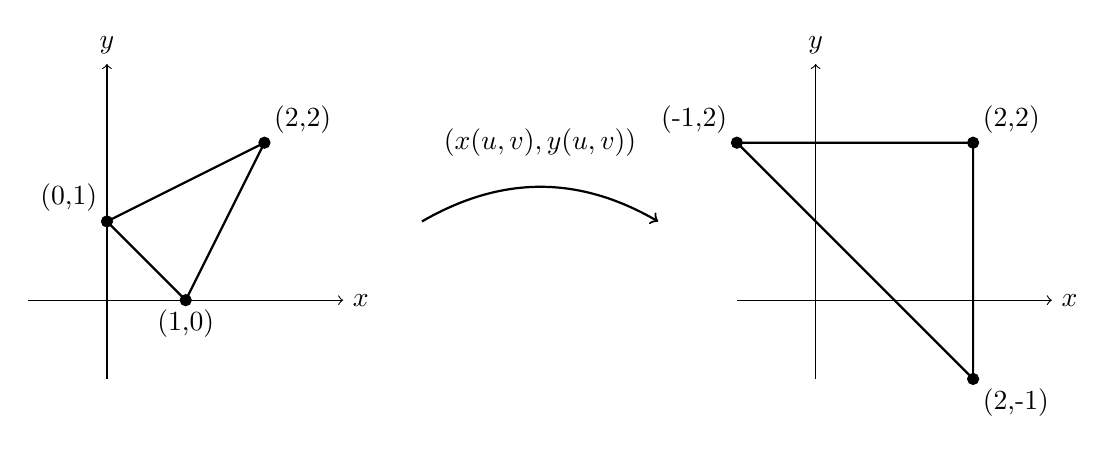
\begin{tikzpicture}
      % draw the xy-axis
      \draw[->] (-1,0) -- (3,0) node[right] {$x$};
      \draw[->] (0,-1) -- (0,3) node[above] {$y$};
      \draw[thick] (0,1) -- (2,2) -- (1,0) -- cycle;

      \filldraw (0,1) circle (2pt) node[above left] {(0,1)};
      \filldraw (2,2) circle (2pt) node[above right] {(2,2)};
      \filldraw (1,0) circle (2pt) node[below] {(1,0)};

      % draw the xy-axis
      \draw[->, shift={(9,0)}] (-1,0) -- (3,0) node[right] {$x$};
      \draw[->, shift={(9,0)}] (0,-1) -- (0,3) node[above] {$y$};

      \draw[thick, shift={(9,0)}] (-1,2) -- (2,2) -- (2,-1) -- cycle;

      \filldraw[shift={(9,0)}] (-1,2) circle (2pt) node[above left] {(-1,2)};
      \filldraw[shift={(9,0)}] (2,2) circle (2pt) node[above right] {(2,2)};
      \filldraw[shift={(9,0)}] (2,-1) circle (2pt) node[below right] {(2,-1)};

      % draw a curved arrow to show the transformation
      \draw[->, thick, bend left=30, shift={(4,0)}] (0,1) to (3,1);
      \node[shift={(4,0)}] at (1.5,2) {$(x(u,v), y(u,v))$};
    \end{tikzpicture}
  \end{figure}
  Therefore, the double integral becomes
  \begin{align*}
    \iint_D (2x - y)^2(2y - x) \,\dA &= \iint_S uv \cdot \left\lVert \frac{\partial (x,y)}{\partial (u,v)} \right\rVert \,\dA \\
                                     &= \frac{1}{3} \int_{-1}^2 \int_{1-u}^2 u^2 v \,\dv \,\du \\
                                     &= \frac{1}{3} \int_{-1}^2 \left[\frac{1}{2}u^2v^2\right]_{1-u}^2 \,\du \\
                                     &= \frac{1}{6} \int_{-1}^2 3u^2 + 2u^3 - u^4 \,\du \\
                                     &= \frac{1}{6} \left[u^3 + \frac{1}{2}u^4 - \frac{1}{5}u^5\right]_{-1}^2 = \frac{33}{20}
  .\qedhere\end{align*}
\end{proof}

\begin{problem}[3]
  Use a change of variable to evaluate $\displaystyle\iiint_E z \,\dV$ where $E$
  is the solid above $z = 0$ and inside $4x^2 + 16y^2 + 8z^2 = 64$.
\end{problem}

\begin{proof}[Solution]
  Let $x = 4u$, $y = 2v$, and $z = \sqrt{8}w$. Then, we get
  \[%
    \frac{x^2}{16} + \frac{y^2}{4} + \frac{z^2}{8} = 1 \implies u^2 + v^2 + w^2 = 1
  .\]%
  The Jacobian of the transformation is
  \[%
    \left\lVert \frac{\partial (x,y,z)}{\partial (u,v,w)} \right\rVert
    = \begin{vmatrix}
      4 & 0 & 0 \\
      0 & 2 & 0 \\
      0 & 0 & \sqrt{8} \\
    \end{vmatrix}
    = 8\sqrt{8} = 16\sqrt{2}
  .\]%
  The bounds are $-1 \le u \le 1$, $-\sqrt{1 - u^2} \le v \le \sqrt{1 - u^2}$,
  and $0 \le w \le \sqrt{1 - u^2 - v^2}$. Converting to spherical coordinates
  gives us the bounds $0 \le \theta \le 2\pi$, $0 \le \phi \le \sfrac{\pi}{2}$,
  and $0 \le 7 \le \rho$. Expanding and evaluating the triple integral gives us
  \begin{align*}
    \iiint_E z \,\dV &= \iiint_S (\sqrt{8}w) \cdot \left\lVert \frac{\partial (x,y,z)}{\partial (u,v,w)} \right\rVert \,\dV \\
                     &= \sqrt{8} \int_0^{2\pi} \int_0^{\sfrac{\pi}{2}} \int_0^1 (\rho\cos(\phi)) \cdot (16\sqrt{2}) \cdot (\rho^2\sin(\phi)) \,\dd{\rho} \,\dd{\phi} \,\dd{\theta} \\
                     &= 64 \int_0^{2\pi} \,\dd{\theta} \cdot \int_0^{\sfrac{\pi}{2}} \cos(\phi)\sin(\phi) \dd{\phi} \cdot \int_0^1 \rho^3 \,\dd{\rho} \\
                     &= 64 \cdot 2\pi \cdot \frac{1}{2} \cdot \frac{1}{4} = 16\pi
  .\qedhere\end{align*}
\end{proof}

\begin{problem}[4]
  Use the change of variable $x = u^2$, $y = v^2$, and $z = w^2$ to express the
  volume of the solid bounded by the surfaces $x = 0$, $y = 0$, and $\sqrt{x} +
  \sqrt{y} + \sqrt{z} = 1$ as an iterated integral in the new variables, $u$,
  $v$, and $w$. It is not required to evaluate the integral.
\end{problem}

\begin{proof}[Solution]
  Finding the Jacobian of the transformation we get
  \[%
    \left\lVert \frac{\partial (x,y,z)}{\partial (u,v,w)} \right\rVert
    = \begin{vmatrix}
      x_u & x_v & x_w \\
      y_u & y_v & y_w \\
      z_u & z_v & z_w \\
    \end{vmatrix}
    = \begin{vmatrix}
      2u & 0 & 0 \\
      0 & 2v & 0 \\
      0 & 0 & 2w \\
    \end{vmatrix}
    = \lvert 8uvw \rvert
  .\]%
  The bounds are $0 \le u \le 1$, $0 \le v \le 1 - u$, and $0 \le w \le 1 - u -
  v$. Expanding the triple integral gives us
  \[%
    V = \int_0^1 \int_0^{1-u} \int_0^{1-u-v} \lvert 8uvw \rvert \,\dw \,\dv \,\du
  .\qedhere\]%
\end{proof}

\begin{problem}[5]
  Evaluate $\displaystyle\int_C 12x \,\ds$ where $C$ is the union of the path $y
  = x^2$ from $(-1, 1)$ to $(2, 4)$ and the line segment between $(2, 4)$ and
  $(3, 2)$.
\end{problem}

\begin{proof}[Solution]
  We integrate over the following two paths, $C_1$ and $C_2$.

  $C_1$: $y = x^2$ from $(-1, 1)$ to $(2, 4)$. This gives us $\r(t) = \langle r,
  r^2 \rangle$ from $t = -1$ to $t = 2$. Therefore, the derivative of the
  position vector is
  \[%
    \r'(t) = \langle 1, 2r \rangle \implies \lvert \r'(t) \rvert = \sqrt{1 + 4t^2}
  .\]%
  Substituting the parameterization into the line integral gives us
  \[%
    I_1 = \int_{-1}^2 12t \sqrt{1 + 4t^2} \,\dt = \left. (4t^2 + 1)^{\sfrac{3}{2}} \right\rvert_{-1}^2 = 17^{\sfrac{3}{2}} - 5^{\sfrac{3}{2}} = 17\sqrt{17} - 5\sqrt{5}
  .\]%

  $C_2$: The line segment between $(2, 4)$ and $(3, 2)$. This gives us $\r(t) =
  \langle 2 + t, 4 - 2t \rangle$ from $t = 0$ to $t = 1$. Therefore, the
  derivative of the position vector is
  \[%
    \r'(t) = \langle 1, -2 \rangle \implies \lvert \r'(t) \rvert = \sqrt{1 + 4} = \sqrt{5}
  .\]%
  Substituting the parameterization into the line integral gives us
  \begin{align*}
    I_2 = \int_0^1 12(2 + t) \sqrt{5} \,\dt = 12\sqrt{5} \int_0^1 2 + t \,\dt = 12\sqrt{5} \left[2t + \frac{1}{2}t^2\right]_0^1 = 12\sqrt{5} \left(2 + \frac{1}{2}\right) = 30\sqrt{5}
  .\end{align*}

  Therefore, the total line integral is
  \[%
    I = \int_C 12x \,\ds = I_1 + I_2 = 17\sqrt{17} + 25\sqrt{5}
  .\qedhere\]%
\end{proof}

\begin{problem}[6]
  Evaluate $\displaystyle\int_C xy \,\ds$ where $C$ is the elliptic helix $x =
  2\cos(t)$, $y = 3\sin(t)$, and $z = t$ for $0 \leq t \leq \sfrac{\pi}{2}$.
\end{problem}

\begin{proof}[Solution]
  We're given the parameterization of the elliptic helix $\r(t) = \langle
  2\cos(t), 3\sin(t), t \rangle$. Therefore, the derivative of the position
  vector is
  \[%
    \r'(t) = \langle -2\sin(t), 3\cos(t), 1 \rangle \implies \lvert r'(t) \rvert = \sqrt{4\sin^2(t) + 9\cos^2(t) + 1} = \sqrt{5} \sqrt{\cos^2(t) + 1}
  .\]%
  Substituting the parameterization into the line integral gives us
  \[%
    \int_C xy \,\ds = \int_0^{\sfrac{\pi}{2}} 6\cos(t)\sin(t) \sqrt{5} \sqrt{\cos^2(t) + 1} \,\dt = 6\sqrt{5}\int_0^{\sfrac{\pi}{2}} \cos(t)\sin(t) \sqrt{\cos^2(t) + 1} \,\dt
  .\]%
  Using $u$-substitution with $u = \cos(t)$ gives us
  \[%
    6\sqrt{5}\int_0^1 u \sqrt{u^2 + 1} \,\du = 6\sqrt{5} \left[\frac{1}{3}(u^2 + 1)^{\sfrac{3}{2}}\right]_0^1 = 6\sqrt{5}\left[\frac{2\sqrt{2}}{3} - \frac{1}{3}\right] = 4\sqrt{10} - 2\sqrt{5}
  .\qedhere\]%
\end{proof}
